\documentclass{sig-alternate-10pt-2013}
\usepackage[usenames,dvipsnames]{color}
\definecolor{mycitegreen}{RGB}{0,90,0}
\definecolor{myrefblue}{RGB}{90,0,0}
\definecolor{cyred}{RGB}{140,0,0}
\definecolor{commentgreen}{RGB}{0,80,0}
\usepackage[draft=true, final=true, colorlinks=true, citecolor=mycitegreen, linkcolor=myrefblue, anchorcolor=myrefblue, pagebackref=false]{hyperref}
\usepackage{graphics,enumitem}
\usepackage{epsfig}
\usepackage{graphicx}
\usepackage{floatrow}
\usepackage[font={bf,small}]{caption}
\usepackage[captionskip=0pt, font={small,bf}, farskip=2pt]{subfig}
\usepackage{multirow}
\usepackage{array}
\usepackage{color}
\usepackage{url}
\usepackage{xspace}
\let\proof\relax
\let\endproof\relax
\usepackage{amsthm}
\usepackage{boxedminipage}

%\usepackage[charter]{template/mathdesign/mathdesign}
%\usepackage{MinionPro}
%\setlength{\textheight}{9.4in}
%setlength{\textheight}{9.25in}
%\setlength{\textwidth}{6.75in}
%\setlength{\columnsep}{.33in}
%\usepackage[]{geometry}

% Compact itemize and enumerate.  Note that they use the same counters and
% symbols as the usual itemize and enumerate environments.
\def\compactify{\itemsep=0pt \topsep=0pt \partopsep=0pt \parsep=0pt}
 \let\latexusecounter=\usecounter
 \newenvironment{CompactItemize}
   {\def\usecounter{\compactify\latexusecounter}
    \begin{itemize}}
   {\end{itemize}\let\usecounter=\latexusecounter}
 \newenvironment{CompactEnumerate}
   {\def\usecounter{\compactify\latexusecounter}
    \begin{enumerate}}
   {\end{enumerate}\let\usecounter=\latexusecounter}

%\baselineskip=12.1bp
%\showthe\baselineskip

\setlength{\pdfpagewidth}{8.5in}
\setlength{\pdfpageheight}{11in}

\makeatletter
\newif\if@restonecol
\makeatother
\let\algorithm\relax
\let\endalgorithm\relax
\usepackage[figure,vlined]{algorithm2e}

\DeclareMathOperator*{\argmax}{arg\,max}

\title{On Consistency in Software Defined Networks}

\numberofauthors{1}
\author{
Paper \#XX, YY pages
}

\begin{document}

\maketitle
%\baselineskip=12bp

% Paragraph Highlight
\newcommand{\paragraphb}[1]{\vspace{0.03in}\noindent{\bf #1} }
\newcommand{\paragraphe}[1]{\vspace{0.03in}\noindent{\em #1} }
\newcommand{\paragraphbe}[1]{\vspace{0.03in}\noindent{\bf \em #1} }

% Comment colors
%\newcommand{\comment}{\textcolor{black}}
\newcommand{\prooffontsize}{\fontsize{8pt}{9.3pt}\selectfont}
\newcommand{\cready}{\textcolor{black}}
\newcommand{\newcomment}{\textcolor{black}}

%\newcommand{\cy}{\textcolor{cyred}{[CY-FIXME]}~\textcolor{cyred}}
%\newcommand{\cycomment}{\textcolor{cyred}}
\newcommand{\cycomment}{\textcolor{black}}
%\newcommand{\matt}[1]{{{#1}}}
%\newcommand{\matt}[1]{{\color{blue}{#1}}}
\newcommand{\matt}[1]{{\color{black}{#1}}}
%\newcommand{\mattc}[1]{{\color{blue}\bf\em{}}}
%\newcommand{\mattc}[1]{{\color{blue}\bf\em{[matt: #1]}}}
\newcommand{\codecomment}{\textcolor{commentgreen}}
%\newcommand{\pbg}{\textcolor{green}}


\newcommand{\swan}{\normalsize S{\small WAN}\xspace}
\newcommand{\swansmall}{\small S{\scriptsize WAN}\xspace}
\newcommand{\cflow}{Vflow\xspace}
\newcommand{\flow}{vflow\xspace}
\newcommand{\flows}{vflows\xspace}

\newcommand{\topolarge}{\textsf{IDN}\xspace}
\newcommand{\toposmall}{\textsf{G-Scale}\xspace}

\newcommand{\corule}{Rule\xspace}
\newcommand{\orule}{rule\xspace}
\newcommand{\orules}{rules\xspace}

\newcommand{\cpr}{Service\xspace}
\newcommand{\pr}{service\xspace}

\newcommand{\cprops}{Service properties\xspace}
\newcommand{\props}{service properties\xspace}

\newcommand{\trurl}{\url{http://somewhere}}

% To make the FIXMEs go away, comment out this line...
\newcommand{\fixme}[1]{{\bf\textcolor{red}{[#1]}}}
% ...and uncomment this one.
%\newcommand{\fixme}[1]{}

\newcommand{\helpme}[1]{{\bf\textcolor{red}{#1}}}

\newcommand{\figtocapskip}{\vspace{-6pt}}
\newcommand{\figtocapbigskip}{\vspace{-9pt}}
%\newcommand{\interfigskip}{\vspace{-12pt}}
%\newcommand{\listskip}{\vspace{-5pt}}
%\newcommand{\listskips}{\vspace{-3pt}}
%\newcommand{\algindent}{\hspace{13pt}}

\theoremstyle{definition}
\newtheorem{lemma}{Lemma}


\begin{sloppypar}
\section{Introduction}
\label{sec:intro}

Software-defined networking (SDN), as envisioned today in separation of control and data planes and centralized control plane computation, is a relatively new concept.
%receiving a lot of attention in the research and practitioner communities.
From early papers (e.g.,~\cite{rcp-case,rcp,4d,ethane}), we learn that its primary promises were $i)$ centralized control plane computation can eliminate the ill-effects (e.g., looping packets) of distributed computation, and $ii)$ separation of control and data planes enables flexible configuration of the data plane in a manner that satisfies a wide range of policy concerns.
For example, the Routing Control Platform (RCP)~\cite{rcp-case,rcp} was motivated by ``oscillations" and ``loops" that can occur in certain iBGP architectures. To avoid these problems, it advocated a centralized control plane that directly configured the data plane of routers in an autonomous system.

4D aimed to simplify network management~\cite{4d}. It observed that the ``data plane needs to implement, in addition to next-hop forwarding, functions such as tunneling, access control, address translation, and queuing." In today's networks, this ``requires complex arrangements of commands to tag routes, filter routes, and configure multiple interacting routing processes, all the while ensuring that no router is asked to handle more routes and packet filters than it has resources to cope with. A change to any one part of the configuration can easily break other parts." Based on this observation, it argues for centrally computing data plane state in a way that obeys all concerns.

Similarly, ETHANE argued that for simplified management of enterprise networks ``policy should determine the path that packets follow"~\cite{ethane}. It then argued for SDNs because the requirements of network management ``are complex and require strong consistency, making it quite hard to compute in a distributed manner." These promises have led to SDNs garnering a lot of attention from the researchers as well as practitioners.

However, as we gain more experience with this paradigm, a nuanced story is emerging.  Researchers have shown that, even with SDNs, packets can take paths that do not comply with policy~\cite{safeupdate} and that more traffic can arrive at a link than its capacity~\cite{swan}. So, what explains this gap between the promise and these inconsistencies. The root cause is that promises apply to the eventual behavior of the network, {\em after} data plane state has been changed and the inconsistencies emerge {\em during} data plane state changes.

Since changes to data plane state, in response to failures, load changes, and policy changes, are an essential part of an operational network, so will be the inconsistencies. Thus, successful use of SDNs requires not only methods to compute policy-compliant data plane state but also methods to change that state in a way that maintains desired consistency properties.

%Going beyond the specific inconsistencies and their solutions considered by prior work~\cite{safeupdate,swan}, this paper presents a broader view of this challenge.

In this paper, we take a broad view of this aspect of SDNs. A basic challenge in consistently updating a network is coordinating rule updates (i.e., changes in data plane state) across multiple switches.  Atomic (i.e., simultaneous) updates to the rules of multiple switches is difficult and uncoordinated updates can lead to inconsistencies such as packet loops and drops. This means that when a given rule can be updated at a switch depends on what rules are present at other switches, and in some cases, these dependencies can be circular.

We consider a spectrum of possible consistency properties, including those in prior work~\cite{safeupdate,swan}, and analyze them with respect to the dependency structures they necessarily induce.
%Through a mix of simple impossibility results and concrete algorithms (some of which are new) from prior work and some we develop),  that can maintain a given consistency property,
We show that dependency structures are simpler for weaker consistency properties and more intricate for stronger properties.  For instance, while maintaining drop freedom (i.e., no packet should be dropped during updates) does not introduce any dependency amongst switches, maintaining packet coherence~\cite{safeupdates} (i.e., no packet should see a mix of old and new rules) makes rules at a switch depend on all other switches in the network.

We also take a detailed view of one particular consistency property---loop freedom, which implies that  no packet should loop during updates---and develop two new update algorithms that induce less intricate dependency structures than currently known algorithms~\cite{safeupdate}. One of our algorithms is provably minimal with respect to the dependencies it induces.

Motivated by the observations of our analysis, we also sketch a general architecture for consistent network updates. This architecture separates across different software modules the two concerns that are primary during network updates: maintaining  consistency and quickly updating the network. Given the consistency property of interest, the first module is responsible for computing a correct plan for updating the network. The update plan is represented as a directed acyclic graph in which nodes are rule updates and edges represent their dependencies.  The second module is responsible for quickly applying the plan based on the properties of the network such as the time it takes for the switches to apply updates and distances between the controller and switches. Preliminary experimental results highlight the value of this architecture as well challenges in implementing it.

\section{Background}
\label{sec:background}

From early papers on SDNs~\cite{rcp-case,rcp,4d,ethane}, we learn that the primary motivations for the SDN paradigm was that centralized computation of network behavior allows us to eliminate the ill-effects (e.g., oscillations and loops) of distributed computation based on partial views and make it easier to compute and implement behaviors that satisfy a wide range of policy concerns. 

For example, consider the Routing Control Platform (RCP)~\cite{rcp-case,rcp}, one of the first proposals that separated the control and data plane of routers. It used a centralized control plane that directly configured the routers in an autonomous system (AS). The primary motivations for this organization were "problems such as protocol oscillations and persistent loops"~\cite{rcp} that can occur in certain iBGP architectures. These problems occur when different routers have different views of network state.

The 4D work has a direct, general argument for an SDN-like architecture~\cite{4d}. It aims to simplify network management. It observes that the "data plane needs to implement, in addition to next-hop forwarding, functions such as tunneling, access control, address translation, and queuing." These functions are implemented using separate processes and it is hard to keep them in sync. "For example, controlling routing and reachability today requires complex arrangements of commands to tag routes, filter routes, and configure multiple interacting routing processes, all the while ensuring that no router is asked to handle more routes and packet filters than it has resources to cope with. A change to any one part of the configuration can easily break other parts." Based on this observation, it argues for centrally computing data plane state in way that obeys all concerns.

ETHANE was aimed at simplifying the management of enterprise networks. It argues that this goal requires, in addition to a high-level policy language and binding packets to their origins, that "policy should determine the path that packets follow." It then employs a centralized control plane, noting that the requirements of network management "are complex and require strong consistency, making it quite hard to compute in a distributed manner."

These promises SDNs have led to them garnering a lot of attention from the research and practitioner communities; however, as we understand this paradigm better, a nuanced story is emerging.  Some researchers have shown that, even when using SDNs, packets can take paths that do not comply with policy~\cite{safeupdate,xx}, and some other researchers have shown that using SDNs can lead to more traffic arriving at a link than its capacity~\cite{swan}.

The gap between the original promises and contradictory behaviors can be explained by the fact that the promised were made about the eventual behavior of the network, {\em after} data plane state has been changed, but the contradictory behaviors occur {\em during} data plane state changes. Since changes to data plane state, in response to failures, load changes, and policy changes, are an essential part of an operational network, so are the contradictory behaviors. Thus, successfully using SDNs means that we not only need flexible means for computing policy-compliant data plane state,  but also need mechanisms to manage changes to the state in a way that complies with policy.

Beyond the specific contradictory behaviors and solutions studies by prior work~\cite{safeupdate,swan}, we present a holistic analysis of such behaviors and what is fundamentally needed to prevent them.

We do not mean to imply that SDNs are not a net positive towards tackling the problems they aim to tackle. We merely wish to highlight that the story (i.e., use centralized computation) is not that straightforward. 

\section{Loop-Free}
\label{sec:example}

\subsection{Example}

\begin{figure}[t!]
\label{fig:example}
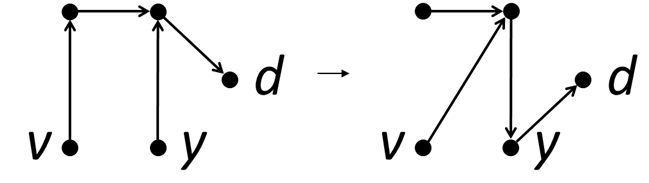
\includegraphics[width=3in]{figures/noloops.png}
\caption{Running example, discussed in Section \ref{sec:example}.}
\end{figure}

Applying routing updates in a way that guarantees no loops is a basic but already interesting consistency property. Consider the five node example network with a single destination $d$ in Figure \ref{fig:example}. The existing routing to destination $d$ on the left of the figure should be updated according to the right of the figure. A naive way to update is to simply send out the forwarding updates (e.g., ``node $u$: for destination $d$ send to $x$''). However, when doing so, it might happen that node $x$ updates its rule before node $y$, introducing a routing loop between nodes $x$ and $y$. This loop will eventually disappear, namely once node $y$ updates its rule, but in an asynchronous system it is difficult to give guarantees when this will happen.

At the other end of the spectrum, the SDN controller could first (i) distribute the new rules, then (ii) wait for an acknowledgement of all the nodes that they have received the new rules, then (iii) tell all the nodes to stop sending packets, and finally, once (iv) they all acknowledged that, (v) tell the nodes to now use the new rules. After the nodes (vi) acknowledge that they are using the new rules, the SDN controller can tell them to (vii) remove the old rules, as they are not needed anymore. This solution does not suffer from loops, as the old and the new solution are well-separated in time.\footnote{Strictly speaking, this protocol is not sufficient, as there might be packets in transit, still using the old rules when rushing through the protocol. Consider a packet sent from sent from $y$ to $x$ shortly before $y$ received the order to stop sending (iii). If node $x$ already passed the last step of the protocol when receiving the packet, node $x$ has not other option then sending the packet back to node $y$, i.e. the packet is experiencing a loop.} However, it is also terribly slow. One may speed up the process by omitting steps (iii) and (iv). Now, assuming that node $x$ received the command to use the new rule (v) earlier than node $y$. As such, in order to guarantee no loop between nodes $x$ and $y$, we must introduce version numbers in packets such that nodes $x$ and $y$ know that packets from $x$ respectively $y$ must be treated according to the new respectively old rules. This is the solution proposed by \ref{theoriginalprincetonpaper}.

One may ask whether version numbers are really necessary, just to guarantee no loops? Also, one may ask whether a faster solution is possible. What nodes are really dependent on each other? This may look like a technicality, but as we all know, nodes are often temporarily unavailable or reacting slowly. If a node must wait for another node, there should better be a consistency reason for it, and not merely protocol overhead. Is there something like a \emph{minimal protocol for a given consistency guarantee}? This is exactly the question we address in this paper.

Regarding our example, the answer to this question is quite simple. Node $u$ does not even need to change its rule, as it always just forwards to $x$, hence node $u$ does not even have to be informed about the rule changes. Node $v$ can switch immediately after being informed about the new rule, as no matter whether using the old or new rule, the packet will always end up at node $x$, with no possibility to experience a loop. Also node $y$ can switch immediately to the new rule, as its packet will then directly reach the destination node $d$. The only critical node in our example is node $x$, for which we understand that node $x$ must wait until node $y$ implemented the switch, as otherwise our network might experience a loop.

More generally, achieving loop-free consistency requires rule updates to wait for each other in a \emph{dependency tree}, i.e., a node may have to wait for one parent node having switched to the new rule before being able to switch itself. Let the destination $d$ be the root of the dependency tree.

We will show two solutions, one with advantages regarding practice as the parent in the dependency forest is always a neighbor node. The practical solution is provably fast, however, it is not optimal regarding dependencies. So, in addition, we also show a more theoretical solution, which (in polynomial time) can compute the minimal dependency forest, i.e. where nodes can switch to the new solution in minimal time.
A node $p$ is a parent of a child node $c$ in the dependency forest if $c$ points to $p$ according to the new rules, e.g. $x$ is a parent of $u$ and $v$. Now, starting at the root, nodes first switch to the new rule, and then inform all their children in the dependency tree to switch as well. Apart from the packets-in-transit problem described above, correctness is immediate: Nodes that are in the dependency tree of the destination will only switch to the new rule once all the nodes on the new path to the destination have already switched. Based on the discussion on the example, it is easy to see that this solution is not minimal, as node $v$ cannot switch immediately, after learning the new rule, but must wait on $x$.


\subsection{Minimal Protocol}

In the following, we will present a protocol which is minimal regarding its dependencies. As the example shows, there may other nodes that can switch immediately. As such the dependency tree turns into a \emph{dependency forest}. As before, in this dependency forest, parents will inform their children when it is safe to use the new rule. The only difference is that the dependency forest is cut to its bare minimum. For simplicity, we first describe the protocol as if there was just a single destination $d$. We then discuss the case where we have multiple destinations.

We need to define \emph{good} and \emph{bad} nodes as follows: The destination $d$ is by definition good. All other nodes $u$ are defined as good or bad regarding the node $v$ at the end of the new forwarding rule \texttt{u.new = v}. If all paths (mixing new and [TODO: still valid] old rules) of $v$ point to the same node $r$ (possibly $r = d$), without loop, then $u$ is good. Else ($v$ has a path that points into a loop) $u$ is bad.

The algorithm to construct the dependency forest is as follows: Initially, we let all good nodes to be roots of the dependency forest. Then, iteratively, while not all nodes are processed, we process an arbitrary good node $u$ by removing its old rule. Removing $u$'s old rule might turn other nodes good; if $v$ turns good when processing $u$, then $v$ is a child of $u$ in the dependency forest.

In the following, we prove a few simple lemmas, which show that (i) the dependency forest is correct and (ii) optimal in the sense that if any node switches to the new rule before the parent in the dependency forest says so, a packet might be experiencing a loop.

Lemma 1: A processed node remains good.

Proof: Since the process only removes old pointers but does not introduce new pointers, new loops cannot will not be introduced during the process, and already good nodes will remain good.

Lemma 2: Every node is eventually processed.

Proof: Take any unprocessed node. We follow the new pointer until we find a pair $u,v$ with \texttt{u.new = v}, $u$ is not yet processed, and $v$ is processed. Since the root of the new pointer in-tree is already processed at the start of the algorithm, and we started at an unprocessed node, such a pair must exist. Because of Lemma 1, node $v$ is good, and as such node $u$ can be processed.

Lemma 3: The process produces a dependency forest.

Proof: Initially good nodes are the roots. If a node $u$ is processed later than a node $v$, then $v$ cannot point to $u$. Listing all the nodes in the order of processing as such only gives parent pointers in one direction, towards the past. As such the produced dependency structure cannot have cycles.

Lemma 4: The process is correct/sufficient (and produces no loops).

Proof: For the sake of contradiction, assume that there is a packet which is sent into a loop. The loop must consist of at least one new pointer, call that \texttt{u.new}, as the old pointers alone do not contain a loop. In other words, node $u$ in the loop deleted its old pointer because it was (and remained, see Lemma 1) good. On the other hand, \texttt{u.new} is on a path that points to node $u$, which is a loop. This is the definition of $u$ being bad. As node $u$ cannot be good and bad at the same time, we have a contradiction.

Lemma 5: The process is optimal/necessary/minimal (no node could flip earlier).

Proof: If nodes can flip immediately, they are by definition optimal, and as such the roots of the dependency forest are optimal. So let us look instead at child node $c$, which must wait for parent $p$ in the dependency tree. Node $c$ becomes good once parent $p$ removes its old pointer, before node $c$ was bad. This means that \texttt{p.old} pointed to a loop, which was removed when \texttt{p.old} was removed. In other words, by definition node $c$ could not switch to the new pointer at any earlier stage, without risking sending a packet on into a loop.

Let us now discuss some of the issues and additional features of this minimal dependency forest. First, what if we update several routes to several (or even all) destinations at the same time. A new rule at a node $u$ may be responsible for a whole prefix $p$ of destinations. In this case, optimality/minimality may be defined in different ways, as some sub-prefixes of prefix $p$ at node $u$ may be good earlier than others. For example, it may be that prefix $p0$ will be good immediately, as it remains unchanged, whereas prefix $p1$ will end up in a loop if we switch immediately. One may now say that the new rule for prefix $p$ should be split up into two rules $p0$ and $p1$, making it possible to switch at least $p0$ immediately. Then the solution above is straight-forward, as we just split up the addressing space into all the minimal sub-prefixes, computing dependency forests for all of them independently. However, even though this solution is in some sense time-minimal, it may be space-inefficient since new rules may now be split up into many sub-prefix rules.

Instead, we may want to define minimality with the original new rules in mind, that is, the new rule of node $u$ for prefix $p$ should not be used before it is loop-free. The concern is that this might lead to deadlocks or sub-optimal time bounds. Indeed, if rules are bundled to meta-rules arbitrarily, one might end up with a deadlock. The canonical example is a triangle network with three nodes and destinations $u,v,w$. The old routing is always clockwise, for two hops. The new routing is counter-clockwise, also for two hops. In other words, in both the old and the new solution, on each of the three links, two destinations are bundled into one rule. Now, no matter which is the three rules is initiated first, we generate a loop for one destination.

In reality, bundling rules is based on prefixes, i.e., rules to different destinations will only be bundled if all destinations share the same prefix. If several rules apply, routing is done according to the longest matching prefix. The example shows that ... this is a problem here, in the most general case! (Yikes, TODO)


-- some old snippets which can be removed --

[TODO: here the old pseudo-code]

Algorithm:
All good nodes u have no parent in the virtual forest, i.e. u.parent = nil, good nodes are ready to be processed.
While not all nodes are processed
	Process an arbitrary good node u: remove the old pointer u.old
	For all bad nodes v:
		If processing u made v good, then v.parent = u

[TODO: Remark: This also works with more than two trees, i.e. with multiple versions of old trees and one new tree. Should I describe a more direct algorithm, an algorithm that does recognize good and bad without calling the Tarjan loop discovery subroutine? What about the failures? In several versions, what happens if a node just does not ack the changes of old versions? Will it become a leaf?]



\begin{table*}[t!]
\begin{center}
\begin{small}
\begin{tabular}{>{\centering\arraybackslash}p{0.7in}|>{\centering\arraybackslash}m{0.75in}|>{\centering\arraybackslash}p{0.8in}|>{\centering\arraybackslash}p{0.85in}|>{\centering\arraybackslash}p{0.85in}|>{\centering\arraybackslash}p{0.75in}|}
&
  \textbf{None}
&
  \textbf{Self}
&
  \textbf{Downstream subset}
&
  \textbf{Downstream all}
&
  \textbf{Global}
\ \\ \hline

  \textbf{Eventual consistency}
&
  Always guaranteed
&
&
&
&
\ \\ \hline

  \textbf{Drop freedom}
&
  \multicolumn{1}{>{\columncolor[gray]{0.8}}c|}{Impossible}
&
  Add before remove
&
&
&
\ \\ \hline

  \textbf{Memory limit}
&
  \multicolumn{1}{>{\columncolor[gray]{0.8}}c|}{Impossible}
&
  Remove before add
&
&
&
\ \\ \hline

  \textbf{Loop freedom}
&
  \multicolumn{2}{>{\columncolor[gray]{0.8}}c|}{Impossible (Lemma \iflongversion \ref{lemma:imp loop-free} \else 6 \fi )}
&
  Rule dep. forest (\S\ref{sec:minimal})
&
  Rule dep. tree (\S\ref{sec:practical})
&
\ \\ \hline

  \textbf{Packet coherence}
&
  \multicolumn{3}{>{\columncolor[gray]{0.8}}c|}{Impossible (Lemma \iflongversion \ref{lemma:imp packet coherence} \else 7 \fi)}
&
  Per-flow ver. numbers
&
  Global ver. numbers~\cite{safeupdate}
\ \\ \hline

  \textbf{Bandwidth limit}
&
  \multicolumn{4}{>{\columncolor[gray]{0.8}}c|}{Impossible (Lemma  \iflongversion \ref{lemma:imp bandwidth limit} \else 8 \fi)}
&
  Staged partial moves~\cite{swan}
\ \\ \hline
\end{tabular}
\end{small}
\end{center}
\vspace{-10pt}
\caption{Some basic consistency properties and their dependencies. Proofs of lemmas are in
\iflongversion
the Appendix.
\else
~\cite{tr}.
\fi
}
\label{tbl:big}
\end{table*}

\section{Consistency space}
\label{sec:table}

Thus far, we have focused on loop freedom; we now take a broader view of the range of consistency properties. Table~\ref{tbl:big} helps frame this view. Its rows correspond to consistency properties. We defined loop freedom and packet coherence in \S\ref{sec:loop-free}; the others are:

\paragraphb{Eventual consistency} No consistency is provided during updates. If the new set of rules computed by the controller are consistent (by any definition), the network will be eventually consistent.

\paragraphb{Drop freedom} No packet should be dropped during update. Drops may occur if a switch lacks a rule to handle a packet and, for scalability, it is not configured to send unmatched packets to the controller~\cite{swan,b4}.

%\item
%\textbf{Loop freedom} There should be no loops during updates, where we define a loop as a packet (without any transformation) visiting an (TODO: ``the same'' instead of ``an''?) interface multiple times.

%\paragraphb{Packet coherence} The set of rules seen by a packet should not be a mix of old and new rules; they should be either all old or all new rules.

\paragraphb{Memory limit} The number of rules that a switch is required to hold is always below a certain limit. A natural limit is the physical capacity of the flow table, but other limits may also be enforced.

\paragraphb{Bandwidth limit} The amount of traffic arriving at a link should not exceed a certain limit. Physical link capacity is a natural limit, but other limits may be interesting as well (e.g., margin for burstiness). That the limit be maintained without dropping traffic is implicit here; otherwise, we can trivially meet any limit.

The consistency properties we list are not the only ones of interest.
%In some applications, one may be happy with eventual consistency, the weakest consistency property possible that just guarantees that eventually, all switches will be following the new rules, and then the network is by definition consistent again.
Some networks may require different properties (e.g., balanced load across two links), and some others may require  guarantees that combine two or more properties (e.g., packet coherence + bandwidth limits). We chose these consistency properties because they are basic and natural, capturing the basic expectations of the experience of packets and network elements.

The consistency properties are listed in rough order of strength, and satisfying a property lower on the list often (but not always) satisfies a property above it. Obviously, packet coherence implies drop and loop freedom (assuming that the old and new rules sets are free of drops and loops). Perhaps less obviously, bandwidth limits imply loop freedom because flows in a loop will likely surpass any bandwidth limit.

However, these properties cannot be totally ordered. Packet coherence and bandwidth limits are orthogonal, as packet coherence does not address bandwidth, and bandwidth limits can be achieved with solutions beyond packet coherence.
Drop freedom and loop freedom are also orthogonal. In fact, trivial solutions for one violates the other---dropping packets before they enter a loop guarantees loop freedom, and just sending packets back to the sender provides drop freedom but creates loops.

%As such we established all relations between the four consistency properties we list in the table.

The columns in Table~\ref{tbl:big} denote dependency structures. They capture rules at which other switches must be updated before a new rule at a switch can be used safely. Thus, the dependency is at the rule level, not switch level; dependencies are often circular at switch level---a rule on switch $u$ depends on a rule on $v$, which in turn depends on $u$ for other rules.
Further, the dependency captures when a new rule can be installed and used safely, not when an old rule can be safely removed. Even after all new rules are being used, the rule set in the network may not be the same as the new rule set; additional (unused) rules may still exist. Such rules will be removed in a clean-up phase. The safe usage time of a new rule is important because it determines when the network is carrying traffic in the new pattern (which may have been necessitated by a failure).


% we will discuss this in \S\ref{sec:discussion}.

The different structures in Table~\ref{tbl:big} are:

\paragraphb{None} The rule does not depend on any other update.

\paragraphb{Self} The rule depends on updates at the same switch.

\paragraphb{Downstream subset} The rule depends on updates at a subset of switches that lie downstream for impacted packets.

\paragraphb{Downstream all} The rule depends on updates at all switches that lie downstream for impacted packets.

\paragraphb{Global} The rule depends on updates even at potentially all switches, including those that are not on the path for packets that use the rule.

%Some characteristics of these dependency properties are worth mentioning. First, note that the dependencies are totally ordered, i.e., no dependency is the weakest, and all is the strongest.


%\ratul{I don't get this: In other words, the dependency categories are on a qualitative level only, and do not give the same insights as a more quantitative understanding on the level of rules. In SWAN \cite{swan}, for instance, progress towards the new solution is achieved in stages, and nodes need to wait with moving to the next stage until other nodes completed the last stage. The goal is to minimize the time until we can use a new solution.}

These dependency structures are qualitative, not quantitative (e.g., time it takes for the update), but in general, update procedures with fewer dependencies (i.e., to the left) are preferable. The cells in Table~\ref{tbl:big} denote whether a procedure exists to update the network with the corresponding consistency property and dependency structure. We can prove that certain combinations are impossible
\iflongversion
(Proofs are in the Appendix.)
\else
\cite{tr}.
\fi
For example, packet coherence cannot be achieved in a way that rules depend on updates at only a subset of downstream switches.

As we can see,  weaker consistency properties (towards the top) need weaker dependency structures (towards the left). At one extreme, eventual consistency (i.e., no consistency during updates) has no dependencies at all.  Slightly stronger properties, drop freedom and memory limit, have dependencies on other rules at the switch itself. A simple procedure for drop freedom is to add the new rule in the switch before the old rule is removed. When installed with higher priority, the new rules become immediately usable, without wait.
%\ratul{should drop freedom be none? there is no dependency on other rules, in terms of when a new rule can be added and used} %not sure that we need anything here, maybe something else that goes into 5?
A simplistic method for maintaining memory limits is to remove an old rule at the same switch before adding the new rule. This method, however, may cause drops or loops.

At the other extreme, maintaining bandwidth limit requires global coordination. The intuition here is that maintaining bandwidth limits at a link requires coordinating all flows that use it, and some of these flows share links with other flows, and so on. Hong et al.~\cite{swan} describe a procedure to effect such transitions by moving flows partially across multiple stages.

Interestingly, all cells to the immediate right of impossible cells are occupied, which implies that, across past work and this paper,  (qualitatively) optimal algorithms for maintain all these consistency properties are known. However, one must not infer from this observation that finding consistent update procedures is a ``solved problem,'' for three reasons. First, some networks may need different properties, for which effective procedures or even best-case structures are unknown (e.g., load balancing across links and maintaining packet ordering within a flow).

Second, even for the properties in Table~\ref{tbl:big}, the picture looks rosy partly because the table focuses on consistency properties in isolation. The combinations are hard to  ensure, and efficient algorithms are not known. For instance, drop freedom and memory limit, while easy to ensure individually, are challenging to ensure in combination. Maintaining the combination requires global dependencies, as introducing some rule at a switch might need to remove another rule first, which can only be removed after having added a new rule somewhere else.

Third, the table only shows the qualitative part of the story, ignoring quantitative effects, which may be equally important. Even though \cite{safeupdate} and \cite{swan} both have global dependencies, \cite{safeupdate} can always resolve the dependencies in two rounds, whereas \cite{swan} may need more stages. Because of these three reasons, we believe that what is presented in this paper is just the tip of iceberg for consistent updates in SDNs.

\section{Discussion}
\label{sec:discussion}

\paragraph{Dependencies vs. time} It is clear that less dependencies improve an update process, as slow or unreachable nodes will slow down less less nodes. However, if all nodes respond timely, less dependence may actually slow down the update process. 

\paragraph{Dependency primitive in switches}

\paragraph{Dependency graphs}


Some additional snippets:

Let’s analyze it. There are only two reasons why we need network algorithms and protocols and the first place, first failures, second changes in either demand or infrastructure; if everything would be stable forever, there is no need to react (have protocols). In this work we essentially concentrate on the second (changes which can be planned). The first is also interesting, but mostly beyond the scope of this work. (This is where Ratul disagrees, and he is probably right.)

Problem: Reaction time to failures and updates. A central controller is often slower than a distributed protocol, as it might be farther away, and the source of the problem/change is often close to those components that are most affected by a problem/change. Nevertheless, that’s again a failure problem. Is the only reason to use distributed protocols failure handling?

(This is what this paper is about.) The answer is no. There is also synchronization. Even in the absence of failures, one cannot have nodes of a network migrate to a new version of operation at the very same instant. In theory, the last statement is trivial. In practice, clearly one tries to get as close as possible to optimal synchronization. Clearly, having an SDN helps a lot, as migration in heterogeneous networks is a whole different battle (this is another thing we discussed), as global updates of standard protocols show. However, even if the system is homogeneous, (time) synchronization is difficult [firing squad, or clock synchronization].

Synchronization is an overloaded term, unfortunately. On the one hand we have something like (physical) clock synchronization, on the other hand we have (logical) synchronization. Perfect physical synchronization is impossible, so people often do logical synchronization. This is also what we do here or in SWAN.

Or, to put it differently, as nodes cannot all migrate to the new version at exactly the same instance (and packets might be in transit still, and what not), we need a way to do a ``save transition'' from the old to the new state.

[Roger removed this missing snippet and used it in 4]

Apart from time, there is also a space component, as we want to remove old rules as soon as possible (as soon as not used anymore).

In this paper we discuss what the ``safe'' in safe transition is.

We also discuss whether there is a tradeoff speed and safety.

We exemplarily look into this tradeoff in one specific example (by looking at different ways to do such a transition).
Some new ideas from discussions:

What helper tools do you have? ``Just control network'' (including gateway routers, but not servers). If needed, one can add header, or mess with TTL. Also: Only talk to neighbors, or able to route messages?

Other consistencies: FIFO, no drop, ``eventual'', suffix.

Worst-case view: If there is a network/traffic pattern with a problem, then the consistency has a problem.

You do not control old and new, so old=new is not a consistency criterion.




{
\scriptsize
%\vspace{5pt}
\baselineskip=7.685bp
\bibliographystyle{abbrv}
\bibliography{paper}
}
%\bibliographystyle{plain}

\end{sloppypar}
\end{document}


